\newpage

\section*{Soluzioni}

\subsection*{Es. 1}
Si riporta sotto il listato del codice richiesto:
%
\lstset{basicstyle=\scriptsize\sf}
\lstinputlisting{./es1/sum0.cpp}
\lstset{basicstyle=\sf}
%
Si noti
che la variabile \cpp{temp} viene distrutta al termine del blocco \cpp{if} all'interno del quale \`e definita. Similmente, la variabile \cpp{i} utilizzata all'interno del ciclo \cpp{for}, non \`e visibile al di fuori di esso. Normalmente si preferisce definire l'indice di un ciclo \cpp{for} all'interno dell'istruzione stessa come mostrato nell'esempio.

Il codice pu\`o essere compilato ed eseguito mediante i comandi seguenti:
\begin{verbatim}
g++ -c sum0.cpp
g++ -o sum0 sum0.o
./sum0
\end{verbatim}
Alternativamente l'istruzione:
\begin{verbatim}
g++ -Wall -o sum0 sum0.cpp
\end{verbatim}
compila il codice e ne fa il \emph{linking} con le librerie statiche.
In sistemi Unix/Linux gli eseguibili non sono riconosciuti in base al
suffisso (\texttt{.exe} in sistemi DOS) e pertanto possono avere
qualsiasi estensione, in questo caso nessuna.
Il parametro \emph{-Wall} permette di stampare
a schermo tutti i ``warning'' (avvertimenti): in questo modo il
compilatore segnala tutto ci\`o che trova di strano nel programma scritto e che
potrebbe essere fonte di errori o problemi. E quindi una buona norma aggiungere
sempre l'opzione \emph{-Wall} e leggere con attenzione i relativi messagi.

Per rispondere al secondo punto \`e sufficiente modificare il tipo
della variabile \cpp{sum} come segue\footnote{Si noti che \cpp{0.} \`e
  un valore di tipo \emph{floating point}, mentre \cpp{0} \`e un
  intero.}:
\begin{lstlisting}
int sum = 0;
\end{lstlisting}
Tentando di calcolare la somma dei quadrati degli interi compresi tra
$1$ e $2000$ si ottiene per la variabile \cpp{sum} il valore
$-1626300296$. La ragione \`e che il valore esatto ($2.66867\cdot
10^9$) risiede al di fuori dei limiti del tipo \cpp{int} (si \`e,
cio\'e, verificato un \emph{integer overflow}). Per comprendere la
ragione per cui il risultato ottenuto \`e negativo, si consideri il
caso di una macchina in cui il tipo intero venga rappresentato con $4$
byte (ovvero \cpp{sizeof(int)} \`e pari a $4$). Il pi\`u grande intero
positivo rappresentabile (2147483647) ha la seguente espressione
binaria:
\begin{equation*}
0\quad 1111111~11111111~11111111~11111111
\end{equation*}
dove si \`e isolato il bit pi\`u significativo, associato al
segno. Sommando $1$ a tale valore otteniamo:
\begin{equation*}
1\quad 0000000~00000000~00000000~00000000
\end{equation*}
che \`e la rappresentazione in complemento di $2$ di $-2147483648$, un
numero negativo. Il massimo ed il minimo valore rappresentabili con un
tipo numerico \cpp{T} sono visualizzabili sull'\emph{output} standard
mediante il seguente comando:
\begin{lstlisting}
std::cout << std::numeric_limits<T>::max() << " , "
          << std::numeric_limits<T>::min() << std::endl;
\end{lstlisting}
%
\begin{figure}
\centering
\psfrag{ldots}{\ldots}
\psfrag{argv}{\cpp{argv}}
\psfrag{chiamata_eseguibile}{chiamata eseguibile}
\psfrag{i}{$i$}
\psfrag{j}{$j$}
\psfrag{argomenti}{argomenti}
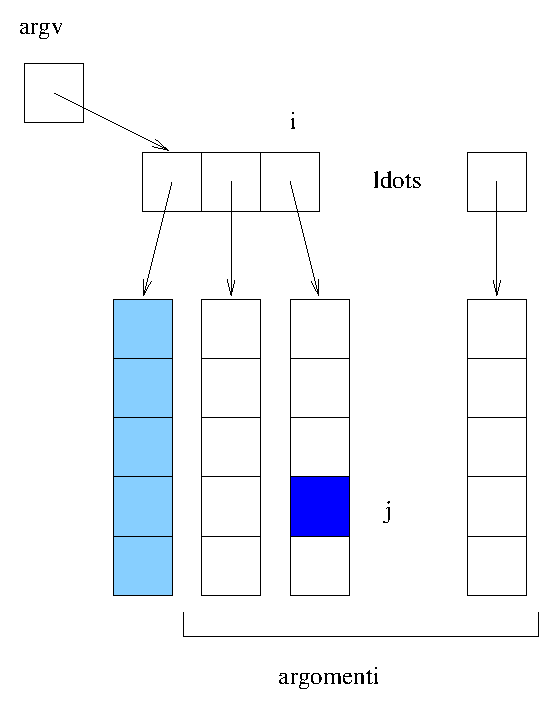
\includegraphics[width=0.4\textwidth]{./figures/eps/argv.eps}
\caption{Schema esplicativo per \cpp{argv}. Il vettore di caratteri in
  azzurro contiene la chiamata all'eseguibile (nel nostro caso
  potrebbe essere ``\texttt{./sum1}''). In blu \`e evidenziato il
  carattere restituito dalla chiamata \cpp{argv[i][j]}, essendo
  \cpp{i} e \cpp{j} due \cpp{int}.}
\label{fig:argv}
\end{figure}
Per rispondere al terzo punto si utilizzano gli argomenti standard
della funzione \cpp{main}, \cpp{argc} e \cpp{argv}. Il primo,
\cpp{argc}, \`e una variabile di tipo \cpp{int} che contiene il numero
degli argomenti introdotti da linea di comando. Il secondo,
\cpp{argv}, \`e vettore di puntatori a stringhe di caratteri (si veda
\figref{fig:argv}). Il primo elemento di \cpp{argv} (di indice $0$)
contiene la chiamata all'eseguibile: sono, perci\`o, disponibili solo
gli argomenti con indice maggiore o uguale a $1$. Poich\'e si vogliono
introdurre due valori numerici, sar\`a necessario convertire le
stringhe di caratteri \cpp{argv[1]} e \cpp{argv[2]} in interi. Per far
ci\`o si pu\`o utilizzare la funzione \cpp{atoi}. Si noti,
incidentalmente, che un vettore di puntatori a stringhe di caratteri
pu\`o essere visto come una matrice di caratteri (si veda ancora
\figref{fig:argv}).
%
\lstset{basicstyle=\scriptsize\sf}
\lstinputlisting{./es1/sum1.cpp}
\lstset{basicstyle=\sf}
%
Si noti inoltre come il comando \cpp{using namespace std}
permetta di evitare di utilizzare il qualificatore \cpp{std::} per
accedere alle classi \cpp{cerr}, \cpp{cout} e \cpp{endl}. Il comando
\cpp{using namespace} deve essere utilizzato con accortezza e solo
quando si \`e sicuri che non vi siano omonimie nei \emph{namespace}
utilizzati.

\subsection*{Es. 2}
Il listato del programma richiesto al primo punto \`e riportato sotto.
%
\lstset{basicstyle=\scriptsize\sf}
\lstinputlisting{./es2/sum1.cpp}
\lstset{basicstyle=\sf}

Si noti che, nell'accesso indiciale, si \`e tenuto conto del fatto
che, in C++, la numerazione degli elementi di un vettore comincia da
$0$.

Il comando \cpp{std::flush} svuota il \emph{buffer} dell'\emph{output
  stream}. \`E opportuno inviarlo allo \emph{stream} quando
l'\emph{output} non termina con un carattere di fine linea
(\cpp{std::endl}).

Una maniera di scorrere il vettore alternativa a quella indiciale \`e
l'utilizzo di un \emph{iterator}. Gli \emph{iterator}, che verranno
discussi approfonditamente nel seguito del corso, sono un'estensione
del concetto di puntatore, utile nella gestione dei contenitori
standard. Gli elementi del vettore \cpp{psum} possono essere stampati
a schermo mediante le seguenti linee di codice:
\lstset{basicstyle=\scriptsize\sf}
\lstinputlisting[linerange={39-41}]{./es2/sum2.cpp}
\lstset{basicstyle=\sf}

 Per scorrere il vettore in senso inverso si pu\`o utilizzare il
 \emph{reverse iterator} associato al tipo \cpp{std::vector<double>}:
\lstset{basicstyle=\scriptsize\sf}
\lstinputlisting[linerange={23-24,42-49}]{./es2/sum3.cpp}
\lstset{basicstyle=\sf}

Si noti che, a differenza di quanto fatto al punto precedente, \`e
stato creato un nuovo tipo psumT mediante il comando
\cpp{typedef}. Tale tipo \`e, in effetti, un \emph{alias} di
\cpp{std::vector<double>}. Un tale accorgimento non solo consente una
maggiore brevit\`a di scrittura, ma evita anche possibili
errori. Qualora, poi, si volesse modificare il tipo per il vettore
delle somme parziali, sarebbe sufficiente ridefinire opportunamente il
tipo derivato \cpp{psumT}. 

La modifica richiesta al terzo punto \`e implementata nelle linee di
codice che seguono e che sostituiscono quelle corrispondenti del
listato al primo punto:
\lstset{basicstyle=\scriptsize\sf}
\lstinputlisting[linerange={24-31}]{./es2/sum2.cpp}
\lstset{basicstyle=\sf}

Se gli elementi fossero stati inseriti mediante il membro
\cpp{operator[]} anzich\'e mediante il membro \cpp{push\_back} avremmo
avuto, al termine, un vettore di misura nulla (\cpp{psum.size() = 0})
e non sarebbe stato possibile accedere alle somme parziali. La ragione
di ci\`o \`e che il membro \cpp{reserve()} riserva la memoria
richiesta, ma non la alloca.

L'assegnamento dei primi dieci elementi di \cpp{psum} pu\`o essere
fatto utilizzando il membro \cpp{assign}, cui vanno passati due
iteratori corrispondenti, rispettivamente, alla prima ed all'ultima
posizione da cui copiare:
\lstset{basicstyle=\scriptsize\sf}
\lstinputlisting[linerange={51-57}]{./es2/sum3.cpp}
\lstset{basicstyle=\sf}

